\documentclass[tikz,border=5pt]{standalone}
\usepackage{tikz}
\usetikzlibrary{positioning,arrows.meta,shapes.geometric,calc,trees}

\begin{document}
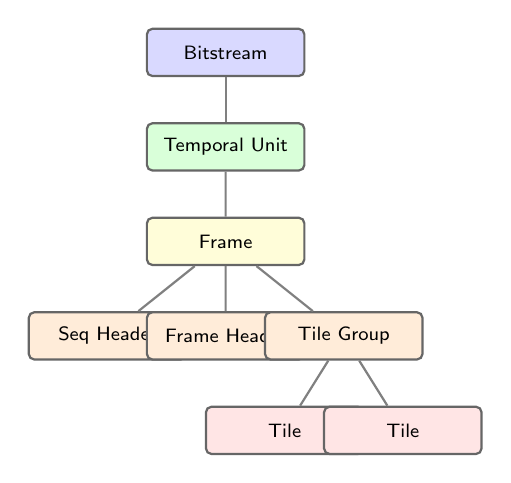
\begin{tikzpicture}[
    level 1/.style={sibling distance=5cm, level distance=1.2cm},
    level 2/.style={sibling distance=2.5cm, level distance=1.2cm},
    level 3/.style={sibling distance=1.5cm, level distance=1.2cm},
    every node/.style={draw=black!60, thick, rounded corners=2pt, minimum width=2cm, minimum height=0.6cm, font=\scriptsize\sffamily, fill=white},
    root/.style={fill=blue!15},
    l1/.style={fill=green!15},
    l2/.style={fill=yellow!15},
    l3/.style={fill=orange!15},
    l4/.style={fill=red!10},
    edge from parent/.style={draw=black!50, thick}
]

\node[root] {Bitstream}
    child { node[l1] {Temporal Unit}
        child { node[l2] {Frame}
            child { node[l3] {Seq Header} }
            child { node[l3] {Frame Header} }
            child { node[l3] {Tile Group}
                child { node[l4] {Tile} }
                child { node[l4] {Tile} }
            }
        }
    };

\end{tikzpicture}
\end{document}
